\chapter{Finite Elements in \texorpdfstring{$d=2$}{d=2}}

\section{Relevant elements}
\subsection{The linear Lagrange element}

If we want to use linear functions, then we must pick $K$ as a triangle.
Let us $z_1, z_2, z_3 \in \mathbb R^d$, and take $K$ as the triangle
\begin{equation}
    \label{eq:FEM d=2 K triangle}
    \trianglegenerated(z_1,z_2,z_3) \defeq \left\{ \sum_{i=1}^3 \theta_i z_i : \theta_i \ge 0 \text{ and } \sum_i \theta_i \le 1\right\}.
\end{equation}
We take $\mathcal P = \mathbb R_1[x]$ and the nodal functions  $N_i (v) = v(z_i)$.

\begin{example}
    Let us take
    \begin{align}
        \label{eq:FEM d=2 K triangle corners}
        z_1 = (0,0) \qquad z_2 = (1,0) \qquad z_3 = (0,1).
    \end{align}
    With this choice we produce the basis of piece-wise linear functions
    \begin{equation*}
        \psi_1 = 1-x-y, \qquad \psi_2 = x, \qquad \psi_3 = y.
    \end{equation*}
\end{example}

\subsection{Quadratic Lagrage elements}

Let us take $K$ the triangle \eqref{eq:FEM d=2 K triangle} and $\mathcal P = Z_2[x]$.
We take $z_1, z_2, z_3$ the vertexes of the triangles and the mid-points $z_4 = \frac{z_2 + z_3}{2}, z_5 = \frac{z_1 + z_3}{2}, z_6 = \frac{z_1+z_2}{2}$. Then $N_i (v) = v(z_i)$.

\subsection{Cubic Hermite triangle}

We take $K$ the triangle \eqref{eq:FEM d=2 K triangle}, $\mathcal P = \mathbb R_3[x]$.
Taking $z_1, z_2,z_3$ the corners of the triangle and $z_4$ the centroid, we define the 10 nodal functions
\begin{equation*}
    \mathcal N = \{ v \mapsto v(z_i): i \in \{1,2,3,4\} \} \cup \left\{v \mapsto \frac{\partial v}{\partial x_k} (z_{i}) : i \in \{1,2,3\} , k \in \{1,2\}\right\}.
\end{equation*}



\subsection{Bi-linear Lagrange rectangle}
We take
\begin{equation}
    K = [0,1] \times [0,1]
\end{equation}
and take $z_1, \cdots, z_4$ the corners of the squares. Take $\mathcal P = \mathbb R_1[x]$ and $N_i(v) = v(z_i)$.

\subsection{Bi-quadratic Lagrange rectangle}
Consider the previous examples and let $z_5, \cdots, z_9$ be the mid-points of the sides. Then we can take $\mathcal P = \mathbb R_2[x]$ and $N_i(v) = v(z_i)$.

\subsection{B-splines}

The B-spline in dimension for a uniform mesh $x_i = (i h, j h )$  can be obtained by tensor product of the one-dimensional B-splines, and we have
\begin{equation*}
    b_{(p_1,p_2),(i,j),h} (x,y) = b_{p_1,i,h}(x) b_{p_2,j,h}(y).
\end{equation*}
Usually $p_1 = p_2 = p$.
For a detailed presentation on splines in higher dimensions see \cite{laiSplineFunctionsTriangulations2007}.

\subsection{Higher-order elements}

There exist a plethora of higher-order elements: Argyris triangle, Hsieh-Clough-Tocher triangle, Singular Zienkievwicz triangle, Veubeke-Sander quadrilateral, ...
An excelent reference is \cite{ciarletFiniteElementMethod2002}.
\Cref{fig:FEM Ciarlet higher order} summarises some higher-order elements
\begin{figure}[p]
    \centering
    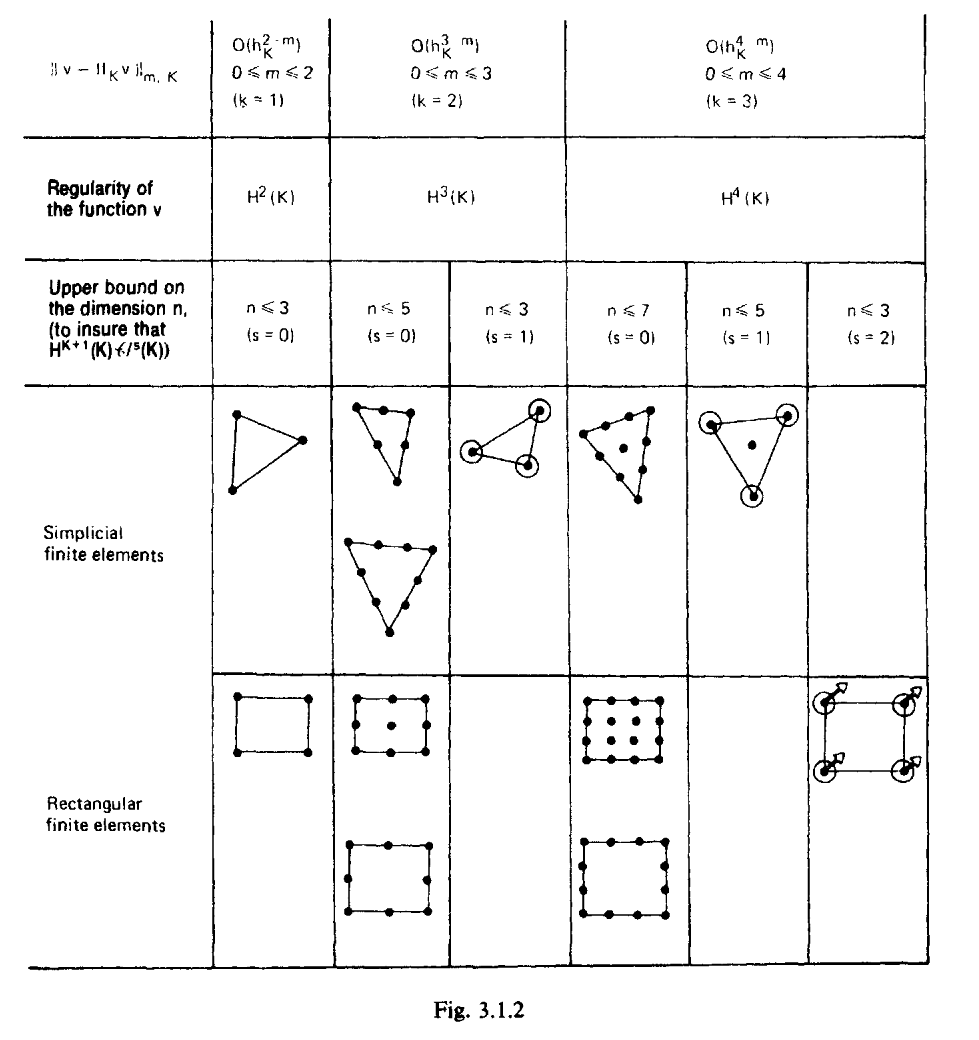
\includegraphics[width=\textwidth]{Ciarlet_diagram}
    \caption{\cite{ciarletFiniteElementMethod2002}. The convention used is that a black indicates that the nodal is obtained by evaluation at that point. A larger circle indicates the derivative is taken at that point.}
    \label{fig:FEM Ciarlet higher order}
\end{figure}

\section{The Dirichlet Laplacian with piece-wise linear basis}

Let $K_0$ be the triangle \eqref{eq:FEM d=2 K triangle} and recall the notation \eqref{eq:FEM d=2 K triangle corners}.
Let $\mathcal T$ be a triangulation of $\Omega$, and let $x_i$ be the corners of the triangles. For each triangle $K \in \mathcal T$ there exists an affine map
\begin{equation*}
    F_K : {K_0} \to  K
\end{equation*}
The space of continuous functions that are linear in each $K$ is generated precisely by the unique continuous piece-wise linear function with value $\varphi_i(x_j) = \delta_{ij}$.
In a triangulation, $\varphi_i \in H^1 (\Omega)$ due to \Cref{thm:H1 glueing}.
In other words, a basis of $\mathcal P_{\mathcal T} \cap C (\overline \Omega)$ is given precisely by
\begin{equation*}
    \varphi_i \Big|_K = \begin{dcases}
        \psi_j \circ F_K^{-1} & \text{if } x_i \in \overline K \text{ and } x_i = F_K z_j \\
        0                     & \text{if } x_i \notin \overline K.
    \end{dcases}
\end{equation*}
It is not difficult to see that these functions are continuous on each $\partial K$, since they are linear.
To include the Dirichlet boundary conditions we take the basis of $\mathcal P_{\mathcal T} \cap H_0^1(\Omega)$ given by
\begin{equation*}
    \mathcal B_{\mathcal T} = \{ \varphi_i : x_i \in \Omega \}.
\end{equation*}

In order to compute the stiffness matrices, we point out that
\begin{equation*}
    \int_\Omega \nabla \varphi_i \cdot \nabla \varphi_j =
    \begin{dcases}
        0
                                    & \text{if } \supp \varphi_i \cap \supp \varphi_j = \emptyset
        \\
        \int_K \nabla \varphi_i \cdot \nabla \varphi_j
                                    & \text{if } i \ne j \text{ and } K = \supp \varphi_i \cap \supp \varphi_j
        \\
        \sum_{\substack{x_i \in \overline K                                                                    \\ K \in \mathcal T}}
        \int_K |\nabla \varphi_i|^2 & \text{if } i = j.
    \end{dcases}
\end{equation*}
Notice that $\nabla \varphi_i$ is constant in each triangle. The computation of the mass matrix is similar, although $\varphi_i$ is not constant.

\subsection{Square triangulation}

Let $\Omega = [0,1] \times [0,1]$ and
consider the mesh $x_{ij} = (ih, ij h)$. We have the sub-division
\begin{equation*}
    \mathcal T =\Big \{ \operatorname{Triangle}( h(i,j), h(i+1,j), h(i ,j+1 )) \Big\} \cup \Big\{ \operatorname{Triangle}( h(i,j), h(i-1,j), h(i ,j-1 )) \Big\}.
\end{equation*}
See \Cref{fig:FEM d=2 triangles on uniform grid}.
\begin{figure}[H]
    \centering
    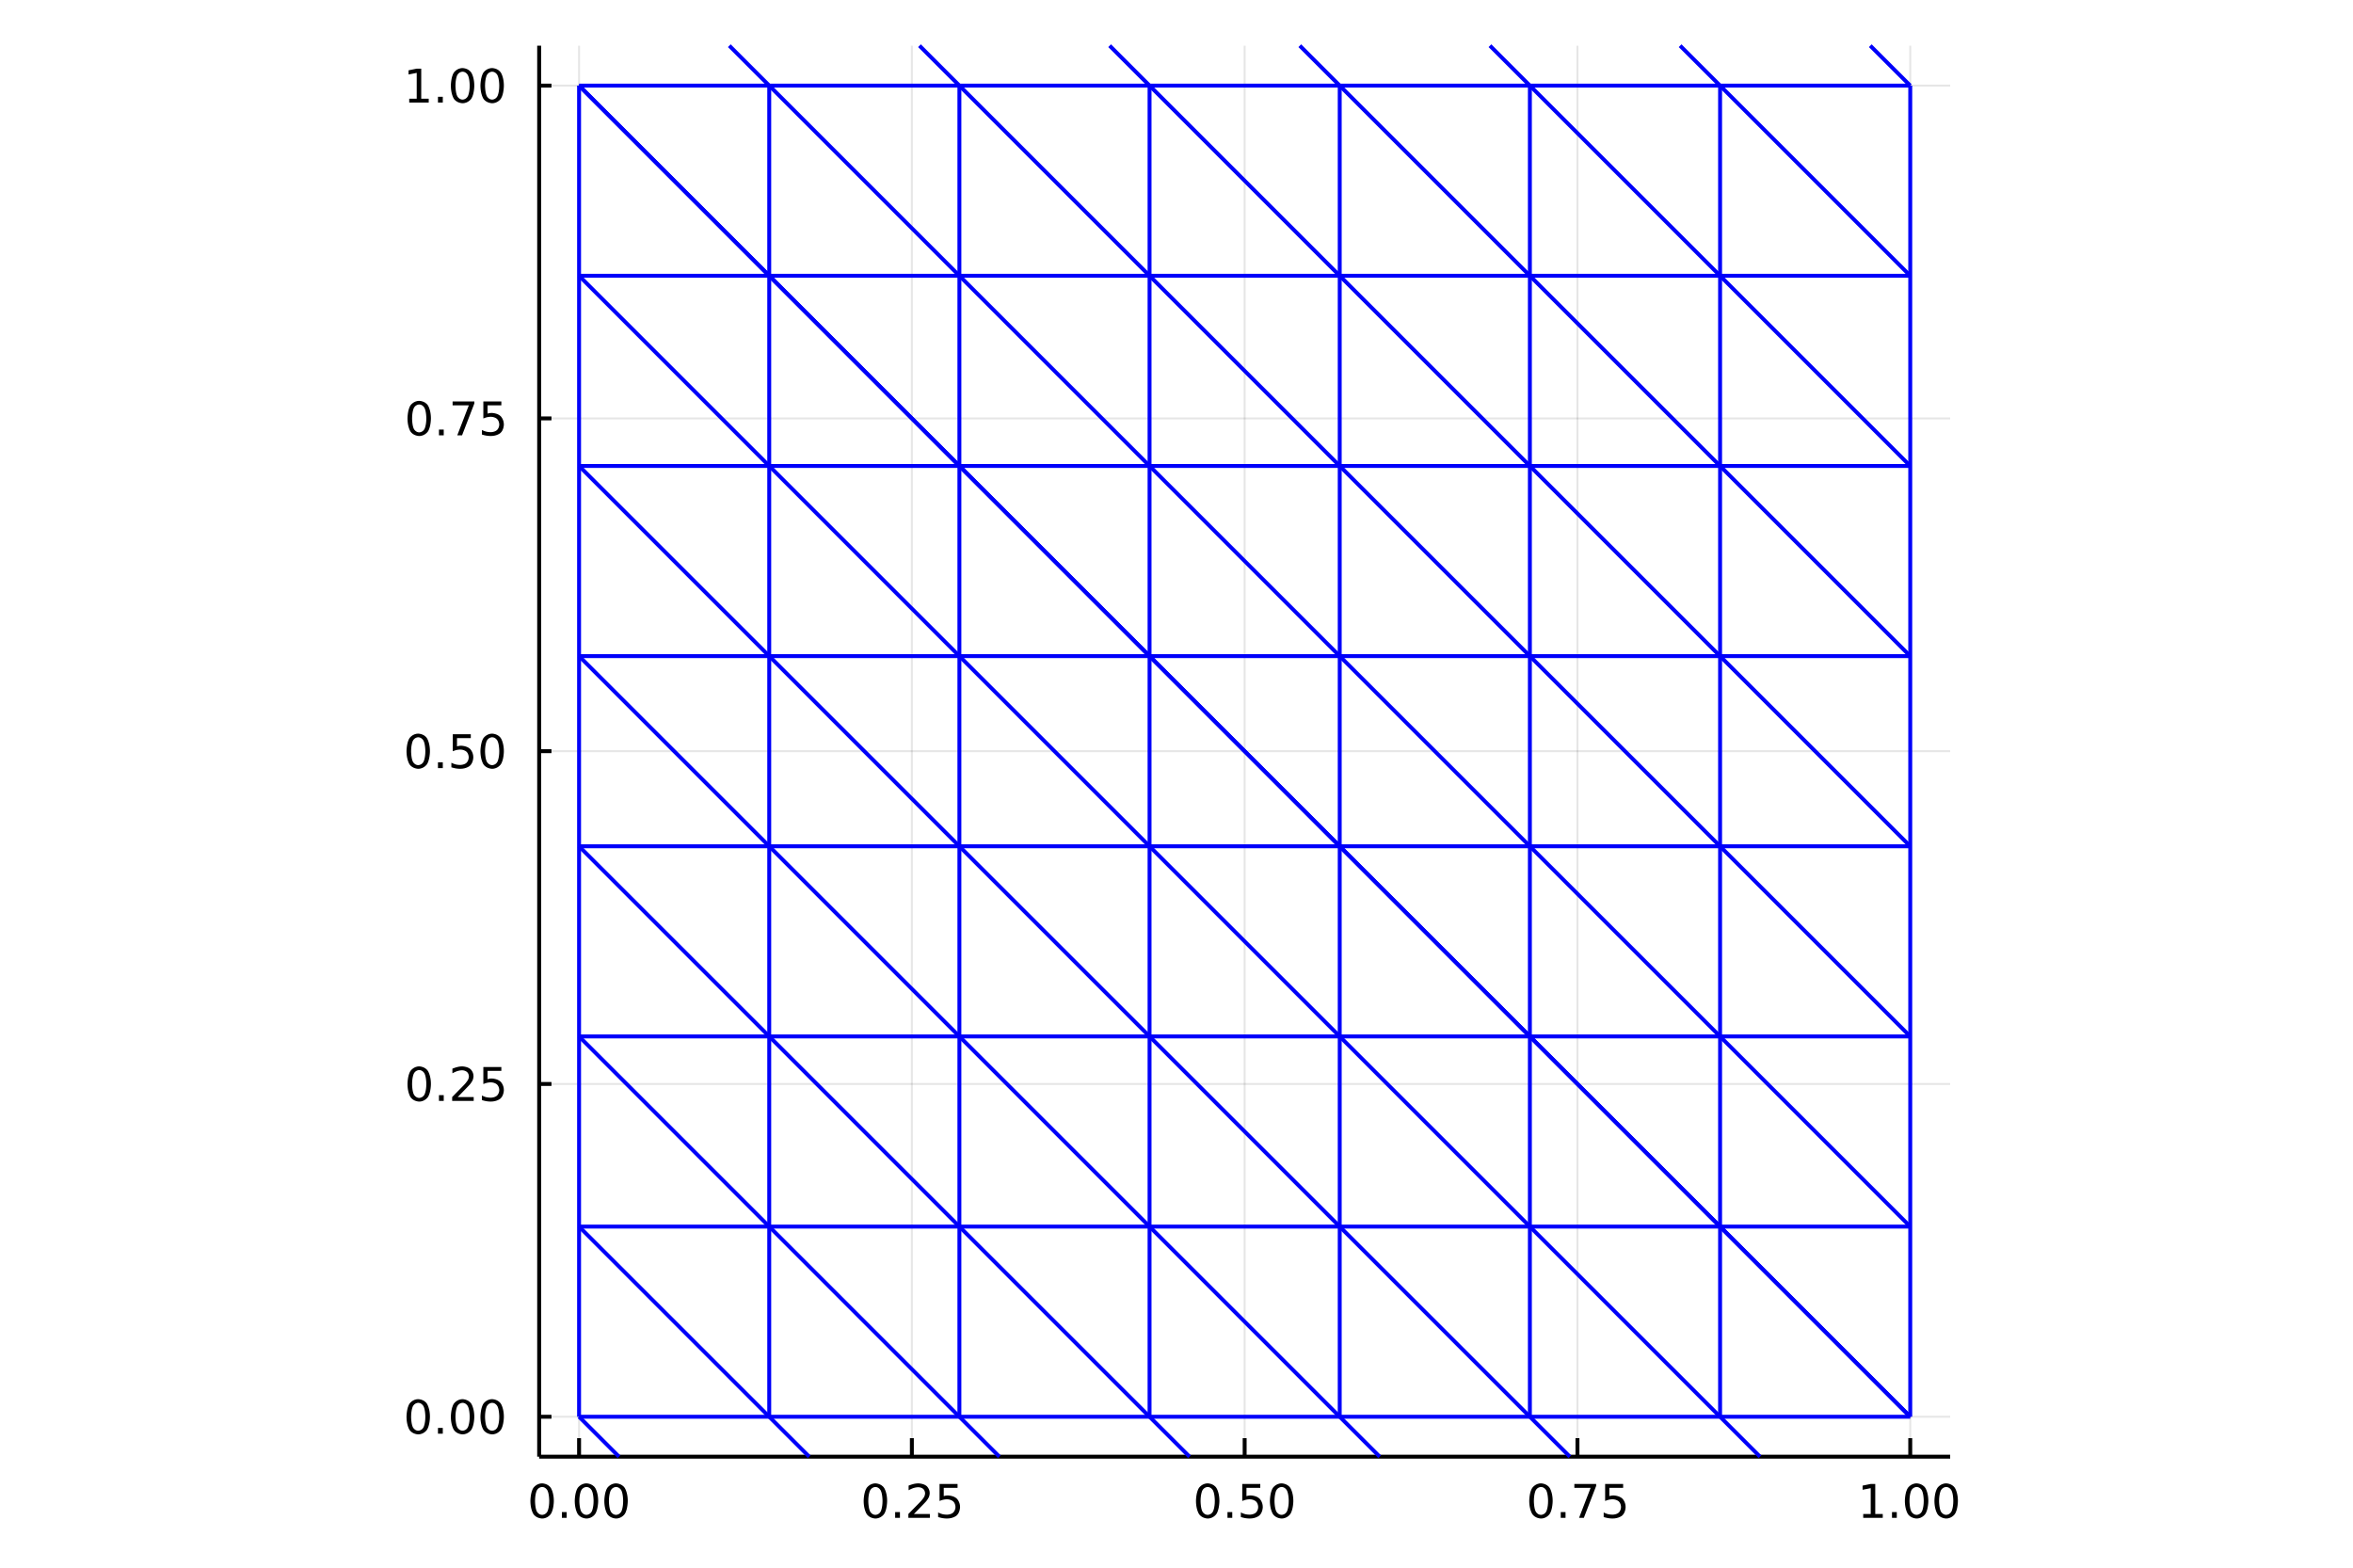
\includegraphics[width=0.5\textwidth]{UniformMesh}
    \caption{Uniform triangulation in dimension $d=2$}
    \label{fig:FEM d=2 triangles on uniform grid}
\end{figure}
We can construct $\varphi_{ij}$ directly. We look at the triangles neighbouring $x_{ij}$ and we get \Cref{fig:FEM d=2 triangles on uniform grid neighbours}
\begin{figure}[H]
    \centering
    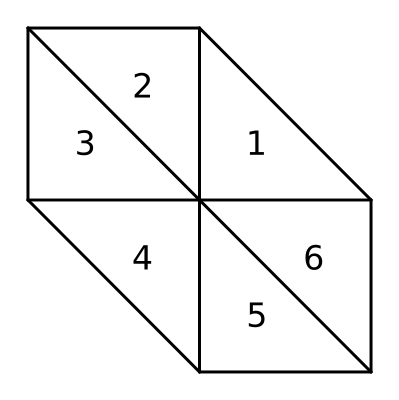
\includegraphics[width=0.25\textwidth]{UniformMesh2}
    \caption{Triangles neighbouring a vertex $x_{ij}$}
    \label{fig:FEM d=2 triangles on uniform grid neighbours}
\end{figure}
We can explicitly write the continuous piece-wise linear function (see \Cref{fig:Piece-wise linear continuous basis function})
\begin{equation*}
    \varphi_{ij} (x,y)
    =
    \begin{dcases}
        1 - \frac{x-x_i}{h} - \frac{y-y_j}{h} & (x,y) \in 1      \\
        1 - \frac{y-y_j}{h}                   & (x,y) \in 2      \\
        1-\frac{x_i-x}{h}                     & (x,y) \in 3      \\
        1-\frac{x_i-x}{h}-\frac{y_j-y}{h}     & (x,y) \in 4      \\
        1-\frac{y_j-y}{h}                     & (x,y) \in 5      \\
        1-\frac{x-x_i}{h}                     & (x,y) \in 6      \\
        0                                     & \text{otherwise}
    \end{dcases}
\end{equation*}
\begin{figure}
    \centering
    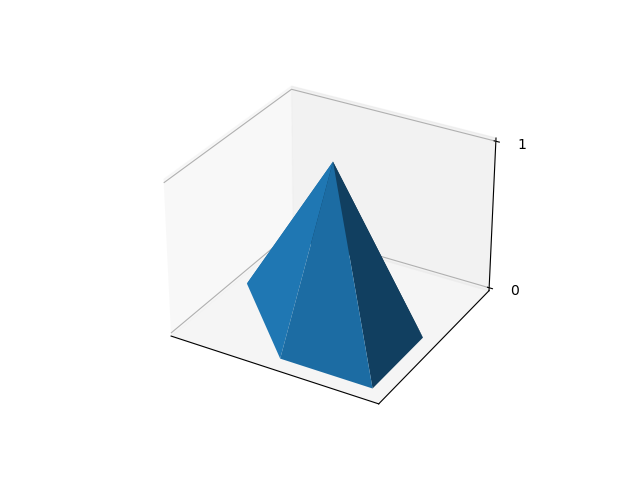
\includegraphics[width=.5\textwidth]{Piramid}
    \caption{A basis function in a square grid. A pyramid.}
    \label{fig:Piece-wise linear continuous basis function}
\end{figure}

Consider
$$
    \begin{dcases}
        -\Delta u = f & Q = [0,1]^2, \\
        u = 0         & \partial Q
    \end{dcases}
$$
and a solution
$$
    u^h(x,y) = \sum_{k,\ell} u_{k,\ell}^h \varphi^h_{k,\ell} (x,y).
$$
Multiplying by a test function we get
$$
    \sum_{k,l} \iint_\Omega U_{kl} \left( \frac{\partial \varphi_{kl}}{\partial x} \frac{\partial \varphi_{ij}}{\partial x}  + \frac{\partial \varphi_{kl}}{\partial y} \frac{\partial \varphi_{ij}}{\partial y}  \right) = \iint_\Omega f \varphi_{ij}  .
$$
The explicit calculation of the integrals leads to
$$
    \frac{-U_{i+1,j} + 2 U_{ij} - U_{i-1,j}}{h^2} + \frac{-U_{i,j+1} + 2 U_{ij} - U_{i,j-1}}{h^2} = \frac{1}{h^2} \iint_{  \textrm{supp} \varphi_{ij}  } f (x,y) \varphi_{ij} (x,y) \diff x \diff y .
$$

Writing this in matrix form is rather inconvenient. It can be achieved concisely using Kronecker products of the finite-difference matrix of dimension $d=1$. We will not get into the details.


\subsection{General triangulation}

In general triangulation there are two approaches to compute the stiffness-matrix.

\paragraph{Direct computation}
Let us consider a triangle of vertexes $(x_i,y_i)$ for $i=1, 2, 3$, then the unique piece-wise linear function such that
$$
    \varphi =
    \begin{cases}
        1 & \text{at } P = (x_1,y_1), \\
        0 & \text{at } Q = (x_2,y_2), \\
        0 & \text{at } R = (x_3,y_3)
    \end{cases}
$$
is given precisely by
$$ \begin{aligned}
        \varphi(x,y; P, Q, R) & = 1
        +
        \frac{y_{2} - y_{3}}{D}\left(x - x_{1}\right)
        + \frac{- x_{2} + x_{3}}{D} \left(y - y_{1}\right) ,
    \end{aligned}
$$
where $D = (x_2-x_1)(y_3-y_1) - (y_2-y_1) (x_3-x_1)$.
The gradient is constant and trivial to compute.

\bigskip

Also if $K$ is a triangle of sides with lengths $a,b,c$ then Heron's formula allows us to compute
\begin{equation*}
    |K| = \sqrt{s(s-a)(s-b)(s-c)}, \qquad s = \frac 1 2 (a + b + c).
\end{equation*}

\paragraph{Via the reference triangle}
For example, for the mass matrix we can compute, if $F_K z_{j_k} = x_{i_k}$ that
\begin{align*}
    \int_K \varphi_{i_1} \varphi_{i_2}
     & = \int_{F(K_0)} (\psi_{j_1} \circ F_K^{-1}) (\psi_{j_2} \circ F_K^{-1}) \\
     & = |\det DF_K| \int_{K_0} \psi_{j_1} \psi_{j_2}.
\end{align*}
The computation of the stiffness matrix is a little more involved, since it will involve multiplying by the constant matrix $DF_K^{-1}$. It is a straight-forward computation with linear functions. This approach is more extensible to general settings.


% The shape functions for two and three dimensional quadratic and cubic B-spline elements are constructed as tensor products of one-dimensional B-splines.

\nocite{Suli}
\printbibliography[heading=subbibliography]